\documentclass[12pt,twoside]{article}

\textwidth 17cm \textheight 25cm \evensidemargin 0cm
\oddsidemargin 0cm \topmargin -2cm
\parindent 0pt
%\parskip \bigskipamount

\usepackage{graphicx}
\usepackage[dutch]{babel}
\usepackage{amssymb,amsthm,amsmath}
%\usepackage{dot2texi}
\usepackage[utf8]{inputenc}
\usepackage{nopageno}
\usepackage{pdfpages}
\usepackage{enumerate}
\usepackage{caption}
\usepackage{wrapfig}
\usepackage{pgf,tikz,pgfplots}
\pgfplotsset{compat=1.15}
\usepackage{color}
\usetikzlibrary{arrows}
\usetikzlibrary{patterns}
\usepackage{fancyhdr}
\pagestyle{fancy}
\usepackage[version=3]{mhchem}
\usepackage{multicol}
\usepackage{fix-cm}
\usepackage{setspace}
\usepackage{mhchem}
\usepackage{xhfill}
\usepackage{parskip}
\usepackage{cancel}
\usepackage{mdframed}
\usepackage{url}
\usepackage{mathtools}
\usepackage{changepage}

\newcommand{\todo}[1]{{\color{red} TODO: #1}}

\newcommand{\degree}{\ensuremath{^\circ}}
\newcommand\rad{\qopname\relax o{\mathrm{rad}}}

\newcommand\ggd{\qopname\relax o{\mathrm{ggd}}}

\pgfmathdeclarefunction{gauss}{2}{%
  \pgfmathparse{1/(#2*sqrt(2*pi))*exp(-((x-#1)^2)/(2*#2^2))}%
}

\def\LRA{\Leftrightarrow}

\newcommand{\zrmbox}{\framebox{\phantom{EXE}}\phantom{X}}
\newcommand{\zrm}[1]{\framebox{#1}}

% environment oefening:
% houdt een teller bij die de oefeningen nummert, probeert ook de oefening op één pagina te houden
\newcounter{noefening}
\setcounter{noefening}{0}
\newenvironment{oefening}
{
  \stepcounter{noefening}
  \pagebreak[0]
  \begin{minipage}{\textwidth}
  \vspace*{0.7cm}{\large\bf Oefening \arabic{noefening}}
}{%
  \end{minipage}
}

\usepackage{calc}

% vraag
\reversemarginpar
\newcounter{punten}
\setcounter{punten}{0}
\newcounter{nvraag}
\setcounter{nvraag}{1}
\newlength{\puntwidth}
\newlength{\boxwidth}
\newcommand{\vraag}[1]{
\settowidth{\puntwidth}{\Large{#1}}
\setlength{\boxwidth}{1.5cm}
\addtolength{\boxwidth}{-\puntwidth}
{\large\bf Vraag \arabic{nvraag} \addtocounter{nvraag}{1}}\vspace*{-0.5cm}
{\marginpar{\color{lightgray}\fbox{\parbox{1.5cm}{\vspace*{1cm}\hspace*{\boxwidth}{\Large{#1}}}}}
\vspace*{0.5cm}}
\addtocounter{punten}{#1}}

% arulefill
\def\arulefill{\leavevmode{\xrfill[-5pt]{0.3pt}[lightgray]\endgraf}\vspace*{0.2cm}}

% \arules{n}
\newcommand{\arules}[1]{
\color{lightgray}
%\vspace*{0.05cm}
\foreach \n in {1,...,#1}{
  \vspace*{0.75cm}
  \hrule height 0.3pt\hfill
}\color{black}\vspace*{0.2cm}}

% \arule{x}
\newcommand{\arule}[1]{
\color{lightgray}{\raisebox{-0.1cm}{\rule[-0.05cm]{#1}{0.3pt}}}\color{black}
}

% \abox{y}
\newcommand{\abox}[1]{
\fbox{
\begin{minipage}{\textwidth- 4\fboxsep}
\hspace*{\textwidth}\vspace{#1}
\end{minipage}
}
}

\newcommand{\ruitjes}[1]{
\definecolor{cqcqcq}{rgb}{0.85,0.85,0.85}
\hspace*{-2.5cm}
\begin{tikzpicture}[scale=1.04,line cap=round,line join=round,>=triangle 45,x=1.0cm,y=1.0cm]
\draw [color=cqcqcq, xstep=0.5cm, ystep=0.5cm] (0,-#1) grid (20.5,0);
\end{tikzpicture}
}


\newcommand{\assenstelsel}[5][1]{
\definecolor{cqcqcq}{rgb}{0.65,0.65,0.65}
\begin{tikzpicture}[line cap=round,line join=round,>=triangle 45,x=#1cm,y=#1cm]
\draw [color=cqcqcq,dash pattern=on 1pt off 1pt, xstep=1.0cm,ystep=1.0cm] (#2,#4) grid (#3,#5);
\draw[->,color=black] (#2,0) -- (#3,0);
%\draw[shift={(1,0)},color=black] (0pt,2pt) -- (0pt,-2pt) node[below] {\footnotesize $1$};
%\draw[color=black] (#3.25,0.07) node [anchor=south west] {$x$};
\draw[->,color=black] (0,#4) -- (0,#5);
%\draw[shift={(0,1)},color=black] (2pt,0pt) -- (-2pt,0pt) node[left] {\footnotesize $1$};
\draw[color=black] (0.09,#5.25) node [anchor=west] {\phantom{$y$}};
%\draw[color=black] (0pt,-10pt) node[right] {\footnotesize $0$};
\end{tikzpicture}
}

\newcommand{\getallenas}[3][1]{
\definecolor{cqcqcq}{rgb}{0.65,0.65,0.65}
\begin{tikzpicture}[scale=#1,line cap=round,line join=round,>=triangle 45,x=1.0cm,y=1.0cm]
\draw [color=cqcqcq,dash pattern=on 1pt off 1pt, xstep=1.0cm,ystep=1.0cm] (#2,-0.2) grid (#3,0.2);
\draw[->,color=black] (#2.25,0) -- (#3.5,0);
\draw[shift={(0,0)},color=black] (0pt,2pt) -- (0pt,-2pt) node[below] {\footnotesize $0$};
\draw[shift={(1,0)},color=black] (0pt,2pt) -- (0pt,-2pt) node[below] {\footnotesize $1$};
\draw[color=black] (#3.25,0.07) node [anchor=south west] {$\mathbb{R}$};
\end{tikzpicture}
}

\newcommand{\visgraad}[1]{\begin{tabular}{p{0.5cm}|p{#1}}&\\\hline\\\end{tabular}}

\newcommand{\tekenschema}[2]{\begin{tabular}{p{0.5cm}|p{#1}}&\\\hline\\[#2]\end{tabular}}

% schema van Horner
\newcommand{\schemahorner}{
\begin{tabular}{p{0.5cm}|p{7cm}}
&\\[1.5cm]
\hline\\
\end{tabular}}

% geef tabular iets meer ruimte
\setlength{\tabcolsep}{14pt}
\renewcommand{\arraystretch}{1.5}

\newcommand{\toets}[3]{
\thispagestyle{plain}
\vspace*{-2.5cm}
\begin{tikzpicture}[remember picture, overlay]
    \node [shift={(15.25 cm,-1.6cm)}] {%
        \includegraphics[width=1.8cm]{/home/ppareit/kaa1415/logokaavelgem.png}%
    };%
\end{tikzpicture}

\begin{tabular}{|llc|c|}
\hline
\vspace*{-0.5cm}
&&&\\
Naam & \arule{4cm} & {\Large\bf KA AVELGEM} & \\
\vspace*{-0.75cm}
&&&\\
Klas & \arule{4cm} & {\Large\bf 20...-...-...} & \\
\hline
\vspace*{-0.75cm}
&&&\\
Toets & {\bf #2} & {\large\bf #1} & Beoordeling\\
\vspace*{-0.75cm}
&&&\\
Onderwerp & \multicolumn{2}{l|}{\bf #3} &\\
\hline
\end{tabular}
}

\newcommand{\oefeningen}[1]{

\fancyhead[LE, RO]{\vspace{0.5cm} #1}
%\thispagestyle{plain}

{\bf \Large \centering Oefeningen: #1}

}

\raggedbottom

\newcommand\vl{\qopname\relax o{\mathrm{vl}}}

\newcommand\dom{\qopname\relax o{\mathrm{dom}}}
\newcommand\ber{\qopname\relax o{\mathrm{ber}}}

\newcommand\mC{\qopname\relax o{\mathrm{mC}}}
\newcommand\uC{\qopname\relax o{\mathrm{{\mu}C}}}
\newcommand\C{\qopname\relax o{\mathrm{C}}}

\newcommand\W{\qopname\relax o{\mathrm{W}}}
\newcommand\kW{\qopname\relax o{\mathrm{kW}}}
\newcommand\kWh{\qopname\relax o{\mathrm{kWh}}}


\newcommand\V{\qopname\relax o{\mathrm{V}}}
\newcommand\ohm{\qopname\relax o{\mathrm{\Omega}}}
\newcommand\kohm{\qopname\relax o{\mathrm{k\Omega}}}


\newcommand\N{\qopname\relax o{\mathrm{N}}}

\newcommand\Nperkg{\qopname\relax o{\mathrm{N/kg}}}

\newcommand\Nperm{\qopname\relax o{\mathrm{N/m}}}

\newcommand\gpermol{\qopname\relax o{\mathrm{g/mol}}}


\newcommand\kgperm{\qopname\relax o{\mathrm{kg/m}}}
\newcommand\kgperdm{\qopname\relax o{\mathrm{kg/dm}}}
\newcommand\gpercm{\qopname\relax o{\mathrm{g/cm}}}
\newcommand\gperml{\qopname\relax o{\mathrm{g/ml}}}


\newcommand{\mA}{\;\mbox{mA}}
\newcommand{\A}{\;\mbox{A}}
\newcommand{\MA}{\;\mbox{MA}}

\newcommand{\us}{\;\mu\mbox{s}}
\newcommand\s{\qopname\relax o{\mathrm{s}}}

\newcommand\h{\qopname\relax o{\mathrm{h}}}

\newcommand{\kmperh}{\;\mbox{km/h}}
\newcommand{\mpers}{\;\mbox{m/s}}
\newcommand{\kmpermin}{\;\mbox{km/min}}
\newcommand{\kmpers}{\;\mbox{km/s}}

\newcommand{\mph}{\;\mbox{mph}}

\newcommand{\Hz}{\;\mbox{Hz}}

\newcommand\Gm{\qopname\relax o{\mathrm{Gm}}}
\newcommand\Mm{\qopname\relax o{\mathrm{Mm}}}
\newcommand\km{\qopname\relax o{\mathrm{km}}}
\newcommand\hm{\qopname\relax o{\mathrm{hm}}}
\newcommand\dam{\qopname\relax o{\mathrm{dam}}}
\newcommand\m{\qopname\relax o{\mathrm{m}}}
\newcommand\dm{\qopname\relax o{\mathrm{dm}}}
\newcommand\cm{\qopname\relax o{\mathrm{cm}}}
\newcommand\mm{\qopname\relax o{\mathrm{mm}}}
\newcommand\um{\qopname\relax o{\mathrm{{\mu}m}}}
\newcommand\nm{\qopname\relax o{\mathrm{nm}}}


\newcommand\Gg{\qopname\relax o{\mathrm{Gg}}}
\newcommand\Mg{\qopname\relax o{\mathrm{Mg}}}
\newcommand\kg{\qopname\relax o{\mathrm{kg}}}
\newcommand\hg{\qopname\relax o{\mathrm{hg}}}
\renewcommand\dag{\qopname\relax o{\mathrm{dag}}}
\newcommand\g{\qopname\relax o{\mathrm{g}}}
\newcommand\dg{\qopname\relax o{\mathrm{dg}}}
\newcommand\cg{\qopname\relax o{\mathrm{cg}}}
\newcommand\mg{\qopname\relax o{\mathrm{mg}}}
\newcommand\ug{\qopname\relax o{\mathrm{{\mu}g}}}
\renewcommand\ng{\qopname\relax o{\mathrm{ng}}}

\newcommand\ton{\qopname\relax o{\mathrm{ton}}}

\newcommand\Gl{\qopname\relax o{\mathrm{Gl}}}
\newcommand\Ml{\qopname\relax o{\mathrm{Ml}}}
\newcommand\kl{\qopname\relax o{\mathrm{kl}}}
\newcommand\hl{\qopname\relax o{\mathrm{hl}}}
\newcommand\dal{\qopname\relax o{\mathrm{dal}}}
\renewcommand\l{\qopname\relax o{\mathrm{l}}}
\newcommand\dl{\qopname\relax o{\mathrm{dl}}}
\newcommand\cl{\qopname\relax o{\mathrm{cl}}}
\newcommand\ml{\qopname\relax o{\mathrm{ml}}}
\newcommand\ul{\qopname\relax o{\mathrm{{\mu}l}}}
\newcommand\nl{\qopname\relax o{\mathrm{nl}}}

\newcommand\MJ{\qopname\relax o{\mathrm{MJ}}}
\newcommand\kJ{\qopname\relax o{\mathrm{kJ}}}
\newcommand\J{\qopname\relax o{\mathrm{J}}}

\newcommand\T{\qopname\relax o{\mathrm{T}}}
\newcommand\uT{\qopname\relax o{\mathrm{{\mu}T}}}

\newcommand\grC{\qopname\relax o{\mathrm{{\degree}C}}}

\newcommand\K{\qopname\relax o{\mathrm{K}}}
\newcommand\calperK{\qopname\relax o{\mathrm{cal/K}}}

\newcommand\hPa{\qopname\relax o{\mathrm{hPa}}}
\newcommand\Pa{\qopname\relax o{\mathrm{Pa}}}

\newcommand\dB{\qopname\relax o{\mathrm{dB}}}

\newcommand\Var{\qopname\relax o{\mathrm{Var}}}

\newcommand{\EE}[1]{\cdot 10^{#1}}

\onehalfspacing

%\setlength{\headsep}{0cm}

\newenvironment{exlist}[1] %
{ \begin{multicols}{#1}
  \begin{enumerate}[(a)]
    \setlength{\itemsep}{0.5em} }
{ \end{enumerate}
  \end{multicols} }




\usepackage{pgfplots}

\usepackage{relsize}


\usepackage{versions}
\excludeversion{theory}


\begin{document}

\pagestyle{fancy}
\lhead{}
\rhead{Oefeningen Reële functies}

\begin{theory}
\thispagestyle{empty}
\begin{center}
  \begin{mdframed}
  \centering
  \fontsize{40}{60}\selectfont Irrationale Functies
  \end{mdframed}
  \vfill
\definecolor{aqaqaq}{rgb}{0.63,0.63,0.63}
\definecolor{wqwqwq}{rgb}{0.38,0.38,0.38}
\begin{tikzpicture}[scale=1.5, line cap=round,line join=round,>=triangle 45,x=1.0cm,y=1.0cm]
\draw[->,color=black] (-3.43,0) -- (3.78,0);
\foreach \x in {-3,-2,-1,1,2,3}
\draw[shift={(\x,0)},color=black] (0pt,2pt) -- (0pt,-2pt) node[below] {\footnotesize $\x$};
\draw[->,color=black] (0,-3.46) -- (0,3.9);
\foreach \y in {-3,-2,-1,1,2,3}
\draw[shift={(0,\y)},color=black] (2pt,0pt) -- (-2pt,0pt) node[left] {\footnotesize $\y$};
\draw[color=black] (0pt,-10pt) node[right] {\footnotesize $0$};
\clip(-3.43,-3.46) rectangle (3.78,3.9);
\draw[line width=1.6pt,color=wqwqwq, smooth,samples=100,domain=-1.9999995090909108:1.999994949917767] plot(\x,{sqrt(4-(\x)^2)});
\draw[line width=1.6pt,color=aqaqaq, smooth,samples=100,domain=-1.9999995090909108:1.999994949917767] plot(\x,{0-sqrt(4-(\x)^2)});
\draw (0.58,2.43) node[anchor=north west] {$f: y=\sqrt{4-x^2}$};
\draw (1.46,-1.5) node[anchor=north west] {$g: y=-\sqrt{4-x^2}$};
\end{tikzpicture}
  \vfill
\end{center}

\subsection*{Doelstellingen}
\vspace*{-0.8cm}
{\singlespacing
Je \hfill  {\scriptsize(LP2006-059, LI1.9, ET32,14,31)}
\begin{itemize}
  \itemsep-0.2em
  \item kan irrationale vergelijkingen oplossen
  \item kan aan de hand van het functievoorschrift een tabel, het domein, de nulwaarden en het tekenverloop bepalen van irrationale functies
  \item kan aan de hand van de grafiek domein, bereik, nulwaarden, tekenverloop, stijgen\&dalen, extrema en asymptotisch gedrag bepalen van irrationale functies
  \item kan vraagstukken/problemen oplossen die aanleiding ge-
ven tot een irrationale vergelijking, ongelijkheid of func-
tie, eventueel met behulp van ICT
  \item kan extremumvraagstukken (ook van buiten de wiskunde)
die aanleiding geven tot irrationale functies, oplossen
\end{itemize}}

\thispagestyle{empty}
\mbox{}
\newpage
\clearpage
\thispagestyle{empty}
%\mbox{}
\tableofcontents
\newpage
\clearpage
\pagenumbering{arabic} 

\fancyhead[RO,LE]{Irrationale functies}
\fancyhead[RE,LO]{}

\end{theory}

\section{Definitie en voorstellingswijze}

\begin{oefening}
Geef twee koppels $(x,y)$ waarvan je weet dat ze niet tot dezelfde functie kunnen behoren.
\end{oefening}

\begin{oefening}
Beschouw een functie met de naam $f$. De argumenten zijn steeds negatieve reële getallen zonder nul en de beelden zijn steeds positieve reële getallen. Noteer $f$ zo expliciet mogelijk.
\end{oefening}

\begin{oefening}
Schrijf de functie met functievoorschrift
$$f:\mathbb{R}\to\mathbb{R}:x\mapsto x^2+x+1$$
nog korter.
\end{oefening}

\begin{oefening}
Schrijf de volgende functies zo kort mogelijk
\begin{enumerate}[(a)]
  \item $f:\mathbb{R}\to\mathbb{R}:x\mapsto \dfrac{1}{x^2+1}$
  \item $f:\mathbb{R}\to\mathbb{R}:x\mapsto 0$
  \item $f:\mathbb{R}\to\mathbb{R}:x\mapsto \sqrt[3]{x^2+1}$
  \item $f:\mathbb{R}\to\mathbb{R}:x\mapsto \left(x^2+1\right)^2$
  \item $f:\mathbb{R}\to\mathbb{R}:x\mapsto x$
\end{enumerate}
\end{oefening}

\begin{oefening}
Beschouw de volgende functies en herschrijf ze als een vergelijking van twee onbekenden
\begin{enumerate}[(a)]
  \item $f:\mathbb{R}\to\mathbb{R}:x\mapsto \sqrt{5+x^3}$
  \item $f:\mathbb{R}\to\mathbb{R}:x\mapsto 3$
  \item $f:\mathbb{R}\to\mathbb{R}:x\mapsto x$
\end{enumerate}
\end{oefening}

\begin{oefening}
Teken met een rode kleur de grafiek van een functie $f$ die door de koppels $(-2, 4)$ en $(2,1)$ gaat. Teken nu met een groene kleur een de grafiek van een andere functie $g$ die door de zelfde koppels gaat.
\end{oefening}

\begin{oefening}
Welke van de volgende grafieken stellen een functie voor?
\begin{center}

\begin{multicols}{2}

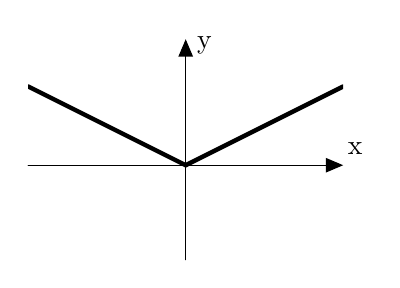
\begin{tikzpicture}[scale=0.2,line cap=round,line join=round,>=triangle 45,x=1.0cm,y=1.0cm]
\draw[->,color=black] (-10,0) -- (10,0);
\draw[color=black] (9.68,0.08) node [anchor=south west] { x};
\draw[->,color=black] (0,-6) -- (0,8);
\draw[color=black] (0.1,7.6) node [anchor=west] { y};
\clip(-10,-6) rectangle (10,8);
\draw [line width=1.6pt,domain=-10.0:0.0] plot(\x,{(-0--2*\x)/-4});
\draw [line width=1.6pt,domain=0.0:10.0] plot(\x,{(-0--2*\x)/4});
\end{tikzpicture}

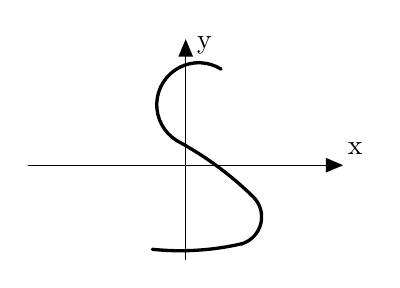
\begin{tikzpicture}[scale=0.2,line cap=round,line join=round,>=triangle 45,x=1.0cm,y=1.0cm]
\draw[->,color=black] (-10,0) -- (10,0);
\draw[color=black] (9.68,0.08) node [anchor=south west] { x};
\draw[->,color=black] (0,-6) -- (0,8);
\draw[color=black] (0.1,7.6) node [anchor=west] { y};
\clip(-10,-6) rectangle (10,8);
\draw [shift={(0.83,3.84)},line width=1.2pt]  plot[domain=1.01:4.16,variable=\t]({1*2.67*cos(\t r)+0*2.67*sin(\t r)},{0*2.67*cos(\t r)+1*2.67*sin(\t r)});
\draw [shift={(-10.73,-17.35)},line width=1.2pt]  plot[domain=0.8:1.08,variable=\t]({1*21.47*cos(\t r)+0*21.47*sin(\t r)},{0*21.47*cos(\t r)+1*21.47*sin(\t r)});
\draw [shift={(3.03,-3.28)},line width=1.2pt]  plot[domain=-1.29:0.84,variable=\t]({1*1.79*cos(\t r)+0*1.79*sin(\t r)},{0*1.79*cos(\t r)+1*1.79*sin(\t r)});
\draw [shift={(-0.34,11.96)},line width=1.2pt]  plot[domain=4.61:4.94,variable=\t]({1*17.39*cos(\t r)+0*17.39*sin(\t r)},{0*17.39*cos(\t r)+1*17.39*sin(\t r)});
\end{tikzpicture}

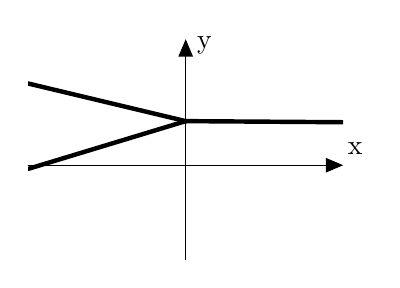
\begin{tikzpicture}[scale=0.2,line cap=round,line join=round,>=triangle 45,x=1.0cm,y=1.0cm]
\draw[->,color=black] (-10,0) -- (10,0);
\draw[color=black] (9.68,0.08) node [anchor=south west] { x};
\draw[->,color=black] (0,-6) -- (0,8);
\draw[color=black] (0.1,7.6) node [anchor=west] { y};
\clip(-10,-6) rectangle (10,8);
\draw [line width=1.6pt,domain=0.0:10.0] plot(\x,{(--8.01-0.02*\x)/2.86});
\draw [line width=1.6pt,domain=-10.0:0.0] plot(\x,{(-10.53-1.14*\x)/-3.76});
\draw [line width=1.6pt,domain=-10.0:0.0] plot(\x,{(-10.08--0.86*\x)/-3.6});
\end{tikzpicture}

\begin{tikzpicture}[scale=0.2,line cap=round,line join=round,>=triangle 45,x=1.0cm,y=1.0cm]
\draw[->,color=black] (-10,0) -- (10,0);
\draw[color=black] (9.73,0.07) node [anchor=south west] { x};
\draw[->,color=black] (0,-6) -- (0,8);
\draw[color=black] (0.09,7.66) node [anchor=west] { y};
\clip(-10,-6) rectangle (10,8);
\begin{scriptsize}
\fill [color=black] (1.46,1.36) circle (4pt);
\fill [color=black] (2.9,2.6) circle (4pt);
\fill [color=black] (4.08,3.96) circle (4pt);
\fill [color=black] (6.2,3.08) circle (4pt);
\end{scriptsize}
\end{tikzpicture}

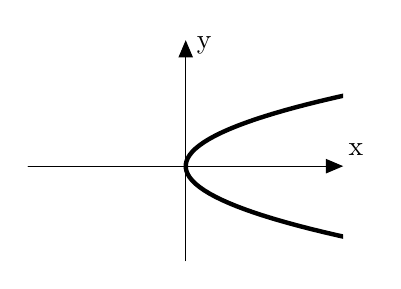
\begin{tikzpicture}[scale=0.2, line cap=round,line join=round,>=triangle 45,x=1.0cm,y=1.0cm]
\draw[->,color=black] (-10,0) -- (10,0);
\draw[color=black] (9.73,0.07) node [anchor=south west] { x};
\draw[->,color=black] (0,-6) -- (0,8);
\draw[color=black] (0.09,7.66) node [anchor=west] { y};
\clip(-10,-6) rectangle (10,8);
\draw [samples=50,rotate around={-90:(0,0)},xshift=0cm,yshift=0cm,line width=1.6pt] plot (\x,{(\x)^2/2/1.0});
\end{tikzpicture}

\begin{tikzpicture}[scale=0.2,line cap=round,line join=round,>=triangle 45,x=1.0cm,y=1.0cm]
\draw[->,color=black] (-10,0) -- (10,0);
\draw[color=black] (9.73,0.07) node [anchor=south west] { x};
\draw[->,color=black] (0,-6) -- (0,8);
\draw[color=black] (0.09,7.66) node [anchor=west] { y};
\clip(-10,-6) rectangle (10,8);
\draw [line width=1.6pt] (3,-6) -- (3,8);
\end{tikzpicture}

\end{multicols}

\end{center}

\end{oefening}


\begin{oefening}
Welke van onderstaande koppels behoren tot de functie met 
$$f:\mathbb{R}\to\mathbb{R}:x\mapsto\frac{6}{x}$$
als functievoorschrift?
\end{oefening}
$$(5,-8)\qquad(-1,4)\qquad(2,3)\qquad(\sqrt{2},\frac{2}{3})\qquad(-6,-1)$$

\begin{oefening}
Geef van een functie met functievoorschrift $f(x)=x^2-4$ een functiewaardentabel die begint bij -5 en eindigt bij 5. Teken daarna de grafiek.
\end{oefening}

\begin{oefening}
Geef van een functie met functievoorschrift $f(x)=\sqrt{x+4}$ een functiewaardentabel die begint bij -5 en eindigt bij 5. Teken daarna de grafiek.
\end{oefening}


\pagebreak
\section{Kenmerken van reële functies}

\begin{oefening}
Beschouw de grafiek van $f$ (de grafiek loopt verder buiten het assenstelsel):\\
\begin{center}
\definecolor{cqcqcq}{rgb}{0.75,0.75,0.75}
\begin{tikzpicture}[scale=0.8,line cap=round,line join=round,>=triangle 45,x=1.0cm,y=1.0cm]
\draw [color=cqcqcq,dash pattern=on 2pt off 2pt, xstep=2.0cm,ystep=2.0cm] (-6.32,-3.09) grid (8.6,4.95);
\draw[->,color=black] (-6.32,0) -- (8.6,0);
\foreach \x in {-6,-4,-2,2,4,6,8}
\draw[shift={(\x,0)},color=black] (0pt,2pt) -- (0pt,-2pt) node[below] {\footnotesize $\x$};
\draw[->,color=black] (0,-3.09) -- (0,4.95);
\foreach \y in {-2,2,4}
\draw[shift={(0,\y)},color=black] (2pt,0pt) -- (-2pt,0pt) node[left] {\footnotesize $\y$};
\draw[color=black] (0pt,-10pt) node[right] {\footnotesize $0$};
\draw[color=black] (6,3) node[right] {$f$};
\clip(-6.32,-3.09) rectangle (8.6,4.95);
\draw[line width=1.6pt, smooth,samples=100,domain=-6.322116381374722:8.604561667405768] plot(\x,{0.01*((\x)+4)*((\x)+1)*((\x)-2)*((\x)-6)});
\end{tikzpicture}
\end{center}
Bepaal (rond af of benader waarden tot één cijfer na de komma):
\begin{itemize}
  \item $\dom f = $\arule{4cm}
  \item $\ber f = $\arule{4cm}
  \item nulwaarden: $x_1=\arule{1.5cm}$, $x_2=\arule{1.5cm}$, $x_3=\arule{1.5cm}$, \arule{3cm}
  \item tekenverloop:\begin{center}\visgraad{6cm}\end{center}
  \item stijgen\&dalen:\begin{center}\visgraad{6cm}\end{center}
  \item extrema:
  \begin{itemize}
    \item absolute maximum: /
    \item relatieve maximum: $y=\arule{1cm}$ bij $x=\arule{1cm}$
    \item absolute minimum: $y=\arule{1cm}$ bij $x=\arule{1cm}$
    \item relatieve minimum: $y=\arule{1cm}$ bij $x=\arule{1cm}$ en $y=\arule{1cm}$ bij $x=\arule{1cm}$
  \end{itemize}
\end{itemize}
\end{oefening}

\begin{oefening}
Teken éérst de grafiek van de functie en bepaal dan net als hierboven de verschillende karakteristieken aan de hand van de grafiek:
\begin{enumerate}[(a)]
  \item $f:\mathbb{R}\mapsto\mathbb{R}: x\mapsto x^2 -4x + 5$
  \item $g: y=\sqrt{x+3}-1$
\end{enumerate}
\end{oefening}

\begin{oefening}
Welke soort veeltermfunctie is het?
\begin{center}
\begin{tabular}{c|c|c|c}
        & Constante & Eerstegraads & Tweedegraads\\
\hline
$\displaystyle f(x)=x$ &&&\\
$\displaystyle f(x)=2$ &&&\\
$\displaystyle f(x)=2x^2-x^2-x^2$ &&&\\
$\displaystyle f(x)=-2x^2+x-4$ &&&\\
$\displaystyle f(x)=0$ &&&\\
$\displaystyle f(x)=4-x$ &&&\\
\end{tabular}
\end{center}
\end{oefening}

\begin{oefening}
Beschouw de functie
$$f(x)=-2x+8$$
en bepaal ervan het domein, het bereik, de nulwaarde(n), het tekenverloop, het stijgen\&dalen en de extrema.
\end{oefening}

\begin{oefening}
Bepaal van de volgende functies
\begin{enumerate}[(a)]
  \item $\displaystyle f(x)=x^2-x-2$
  \item $\displaystyle f(x)=-x^2+6x-5$
  \item $\displaystyle f(x)=x^2-8x+16$
  \item $\displaystyle f(x)=-x^2-2x+3$
\end{enumerate}
het domein, het bereik, de nulwaarde(n), het tekenverloop, het stijgen\&dalen en de extrema.
\end{oefening}



\pagebreak
\section{Symmetriën}

\end{document}




\begin{minipage}[c]{0.4\textwidth}
\end{minipage}
\begin{minipage}[c]{0.6\textwidth}
\dotlines{10}
\end{minipage}




















